
\subsubsection{Chemical Treatment}
Chemical substances are utilized to remove contaminants from 
the glass or to modify its surface state to be more suitable 
for bonding. These processes are categorized as \textit{Chemical Cleaning} 
and \textit{Chemical Activation}, respectively.
\\\\
The most common chemicals used for cleaning include:
\begin{itemize}
\item \textbf{Detergents and Solvents} 
\begin{itemize}
\item \textbf{Micro-Soap:} Eliminates heavy organic matter and 
        solid particles by reducing the surface tension of the water. 
        This allows contaminants to detach from the glass surface, making 
        them easier to remove during rinsing.
\item \textbf{Acetone:} Effectively dissolves fats, waxes, and 
        photoresists by breaking down organic polymer chains.
\item \textbf{Ethanol:} Typically used as the final solvent cleaning 
        step, as it removes residual chemicals and water. Its high volatility 
        ensures it evaporates quickly, leaving the surface ready for subsequent 
        treatments such as acid baths or plasma activation.
\end{itemize}
\item \textbf{Stronger Chemicals} 
\begin{itemize}
\item \textbf{Piranha Solution:} A mixture of Sulfuric Acid ($H_2SO_4$) and 
        Hydrogen Peroxide ($H_2O_2$). It is extremely corrosive and oxidizing, 
        making it the standard for removing stubborn organic residues.
\item \textbf{RCA-1:} A solution of Ammonium Hydroxide, Hydrogen Peroxide, 
        and water. It removes light organic films and dislodges insoluble particles 
        from the glass surface through electrostatic repulsion.
\item \textbf{RCA-2:} A mixture of Hydrochloric Acid, Hydrogen Peroxide, 
        and water used to eliminate heavy metals and alkaline contaminants.     
\end{itemize}
\end{itemize}
In the case of Fused Silica or Quartz glass ($SiO_2$), surface activation consists 
of increasing the density of hydroxyl groups (-OH) on the surface. This creates 
silanol groups (Si-OH), which are essential for successful bonding~\cite{CITA}. When 
two surfaces populated with silanol groups are brought into contact, hydrogen bonds 
are established between them~\cite{CITA}. While these bonds do not initially generate 
a high-strength joint, they serve as the necessary precursor for permanent covalent 
bonds, which are finalized through thermal treatment, as detailed in the \textit{Thermal Treatment} 
section. A summary of this process is illustrated in Figure~\ref{fig:bonding_process1}. 
Generally, surface activation is achieved by soaking the glass in RCA-1 or through 
plasma treatment.
\\\\
To maximize the efficiency of these chemical treatments, the use of ultrasonic cleaners
is highly recommended during the initial cleaning stages. These devices utilize high-frequency 
sound waves to create microscopic vacuum bubbles in the liquid ---a process known as \textit{cavitation}. 
The implosion of these bubbles near the glass surface provides a mechanical scrubbing 
action that removes sub-micron particles and contaminants from pores that are otherwise 
inaccessible to standard chemical soaking.
\begin{figure}[h]
\centering
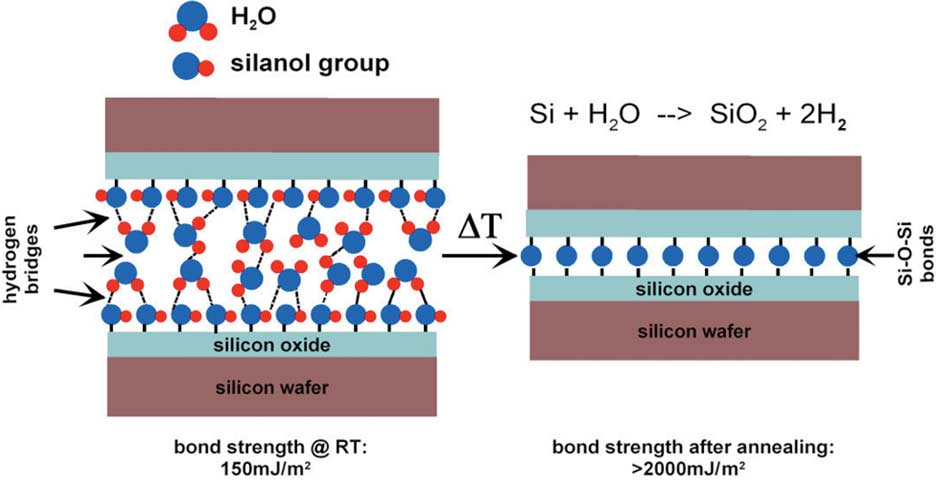
\includegraphics[width=\textwidth]{Images/bonding_process.jpg}
\caption{Bonding process of two Fused Silica surfaces. Initially,
    hydrogen bonds are formed between them due to the presence
    of Silanol (Si-OH) groups. These bonds are subsequently transformed into 
    stronger covalent bonds through thermal treatment.}
\label{fig:bonding_process1}
\end{figure}

